% sage_latex_guidelines.tex V1.10, 24 June 2016

\documentclass[Afour,sageh,times]{sagej}

% customizations
\usepackage[super]{nth}
\usepackage[inline]{enumitem}
\usepackage{moreenum}
\usepackage{tabulary}
\usepackage{tabu}
\usepackage{booktabs}
\usepackage{array}
\usepackage[super]{nth}
\usepackage{listings}
\usepackage{float}
\usepackage{tikz}
\usepackage{upquote}
\usepackage{graphicx}
\usepackage{epstopdf}
\usepackage{tabularx}
\usepackage{newclude}
\newcolumntype{Y}{>{\raggedright\arraybackslash}X}
\newcommand{\ra}[1]{\renewcommand{\arraystretch}{#1}}

% special characters
\usepackage{gensymb}
\usepackage{amssymb}
\usepackage{pifont}
\newcommand{\cmark}{\ding{51}}
\newcommand{\xmark}{\ding{55}}

% sage packages and commands
\usepackage{moreverb,url}
\usepackage[colorlinks,bookmarksopen,bookmarksnumbered,citecolor=red,urlcolor=red]{hyperref}
\newcommand\BibTeX{{\rmfamily B\kern-.05em \textsc{i\kern-.025em b}\kern-.08em
T\kern-.1667em\lower.7ex\hbox{E}\kern-.125emX}}


% ---------------------------- METADATA ---------------------------- 

\def\volumeyear{2017}
\begin{document}
\runninghead{Harmon et~al.}
\title{Tangibly modeling landscapes}
%\title{Tangible Landscape}
%\title{Tangible Landscape Architectural Modeling}
%\title{Tangible Landscape Modeling}
\author{Brendan A Harmon\affilnum{1,2}, Anna Petrasova\affilnum{1}, Vaclav Petras\affilnum{1}, Helena Mitasova\affilnum{1}, and Ross Meentemeyer\affilnum{1}}
\affiliation{\affilnum{1}Center for Geospatial Analytics, North Carolina State University, USA\\
\affilnum{2}College of Design, North Carolina State University, USA}
\corrauth{Brendan A Harmon, 
Center for Geospatial Analytics,
North Carolina State University,
Raleigh, NC 27615, USA.}
\email{brendan.harmon@gmail.com}

% ---------------------------- ABSTRACT ---------------------------- 

\begin{abstract}
We present Tangible Landscape 
-- a technology for rapidly and intuitively designing landscapes
informed by geospatial modeling, analysis, and simulation.
%
Tangible Landscape is a tangible interface powered by a geographic information system 
that gives 3D spatial data an interactive, physical form so that 
users can naturally sense and shape it.
%
It couples a physical and a digital model of a landscape
through real-time cycles of 
physical manipulation, 3D scanning, spatial computation, and projected feedback.
% 
Natural 3D sketching and real-time analytical feedback should aid
landscape architects in the design of high performance, process-based landscapes.
%
We conducted a series of studies to assess the effectiveness of 
tangible modeling for landscape architects.
%
Landscape architecture students, academics, and professionals 
were given a series of fundamental landscape design tasks 
-- topographic modeling, cut-and-fill analysis, and water flow modeling. 
%
Their performance was assessed using both qualitative and quantitative methods.
%
With tangible modeling the participants
effectively modeled topography and water flow 
producing more accurate models 
that better represented morphological features 
than they did with either digital or analog, hand modeling.
%
When tangibly modeling
they used a rapid, iterative process informed by geospatial analytics 
that enhanced their performance.  
\end{abstract}

\keywords{Human-computer interaction, tangible interfaces, embodied cognition, geospatial modeling, topographic modeling, hydrological modeling}

\maketitle

% ---------------------------- INTRO ---------------------------- 

\section{Introduction}

% GIS IN LANDSCAPE ARCHITECTURE
Landscape architects use 
geographic information systems (GIS) to map and analyze landscapes
and computer aided design (CAD) software % 3D modeling software
to computationally represent and design landscapes.
%
While GIS can quantitatively model, analyze, simulate, and visualize 
complex spatial and temporal phenomena,
these systems can be unintuitive, challenging to use, and creatively constraining
due to the complexity of the software, 
the complex workflows, 
and the limited modes of interaction and visualization 
\cite{Ratti2004}. 
%
Due to the complex, time consuming workflows 
needed to link geospatial analysis with computer aided design 
GIS tends to play a limited, often preliminary role in the creative design process.
%
While GIS has been used extensively in landscape planning 
to model scenarios \cite{Steinitz2004,Baker2004,Steinitz2012},
in landscape architecture
it is primarily used for preliminary research and mapping.
%
If, however, geospatial analysis, modeling, and simulation
could be seamlessly integrated into the creative design process 
then designers could rapidly develop design ideas
while quantitively testing them. 
%
In such a rapid, fluid creative process
the rigorous testing of design concepts 
with quantitive measures of performance 
could drive the development of new concepts.
%
Simulation for example could inspire ideation 
linking designed form with environmental processes. 

% TANGIBLES
When using a graphical user interface (GUI) 
-- the paradigmatic mode of interaction for both CAD and GIS --  
intention is translated from physical input 
using devices like a mouse and keyboard 
to digital data rendered visually as text and graphics. 
%
Positing that graphical interaction is unintuitive
because of this disconnect between 
intention, physical action, and purely visual feedback,
researchers have been developing tangible user interfaces 
to give digital data interactive physical form 
\cite{Dourish2001,Ishii2008}. 
%
Theoretically tangible interfaces should embody cognition 
-- grounding higher cognitive processes in bodily experience --
by enabling users to kinaesthetically sense and interact with digital data
\cite{Kirsh2013}.
%
Tangible, embodied interaction should be highly intuitive 
since it 
uses existing motor schemas,  
offloads cognitive work onto the body,
and seamlessly connects intention, action, and feedback.

% TANGIBLES FOR LANDSCAPE ARCHITECTURE
The MIT Media Lab developed two prototypes 
-- Illuminating Clay and SandScape -- 
that coupled a physical and digital model of a landscape
through a cycle of 3D scanning, geospatial computation, and projection
to combine the affordances of intuitive sculpting by hand
with quantitative geospatial analysis \cite{Piper2002a}. 
%
These systems were designed to 
'streamline the landscape design process 
and result in a more effective use of GIS, 
especially when distributed decision-making and discussion 
with non-experts are involved' \cite{Ratti2004}.
%
Recent advances in sensors and computer vision
have fueled the development of 
%new tangible interfaces including systems 
systems for tangibly modeling landscapes such as 
Efecto Mariposa \cite{Vivo2011} and
the Augmented Reality Sandbox \cite{Kreylos2012,ARsandbox}, 
Sedimachine \cite{Cantrell2014}, and
the Rapid Landscape Prototyping Machine \cite{Robinson2014}.

\subsection{Tangible Landscape}
Inspired by Illuminating Clay, 
the Tangible Geospatial Modeling System 
\cite{Mitasova2006,Tateosian2010}, 
and the Augmented Reality Sandbox, 
we have develop Tangible Landscape 
-- a tangible interface for geospatial modeling
powered by an open source GIS \cite{Petrasova2015}. 
%
% TL premise: algorithmic design of landscapes
% Conceptually Tangible Landscape is meant to... 
%
With Tangible Landscape
designers can sculpt a terrain model in polymeric sand,
and can digitize points, areas, and volumes by placing 
color-coded markers, patches of felt, or building blocks. 
%
These interactions are captured by a Kinect sensor, 
processed in GRASS GIS, 
and the resulting geospatial computations
are projected back onto the physical model, 
all in real-time (Fig.~\ref{fig:system_diagram}).
%
The geospatial data can also be automatically
3D modeled and rendered in Blender 
on a monitor or head-mounted display
so that designers can 
immersively explore different views \cite{Tabrizian2016}.
%
For example
as users sculpt topography,
simulated water flow can be projected back onto the model in real-time
so that they understand how they are affecting 
physical processes in landscape.
Then as they draw planting areas 
using a laser pointer or patches of colored felt,
the trees can be rendered in 3D on a display %. 
%As they place markers to designate waypoints on a trail,
%the optimal walking route can be computed and projected onto the model
%along with charts showing metrics like distance and slope
(Fig.~\ref{table:tl_demo}). 

Tangible Landscape 
is unique since it powered by a GIS
with extensive libraries for geospatial computation
and has a wide range of real-time interactions including 
3D sculpting, 3D sketching, color recognition, and object recognition.
%
Given its versatility 
there are many possible design applications
including terrain modeling, hydrological modeling, flood prevention,
trail planning, viewshed analysis, and planting design. 

% TL DIAGRAM
\begin{figure}
    \begin{center}
        \includegraphics[width=0.45\textwidth]{images/diagrams/rendered_diagram_2.pdf}
        %\includegraphics[width=0.25\textheight]{images/diagrams/rendered_diagram_2.pdf}
        %\includegraphics[width=0.32\textheight]{images/diagrams/rendered_diagram_3.pdf}
        \caption{Tangible Landscape: a real-time cycle of 3D scanning, geospatial computation and 3D modeling, and 3D rendering and projection.}
        \label{fig:system_diagram}
    \end{center}
\end{figure}

% TL DEMO
\begin{table*}
\caption{Collaboratively sculpting topography to create lakes, drawing trees with a laser pointer, and visualizing with 3D renderings.} %Source: \cite{Tabrizian2016}.
\ra{1.3}
\begin{tabular}{m{0.49\textwidth} m{0.49\textwidth}}
\toprule
\multicolumn{1}{c}{Sculpting}  & \multicolumn{1}{c}{Drawing and visualization}\\
\midrule
%
\includegraphics[width=0.49\textwidth]{images/immersive/sculpting_lakes_2.png} &
\includegraphics[width=0.49\textwidth]{images/immersive/drawing_trees_1.png}\\
%
\includegraphics[width=0.49\textwidth]{images/immersive/sculpting_landforms_2.png} &
\includegraphics[width=0.49\textwidth]{images/immersive/drawing_trees_2.png}\\
%
\includegraphics[width=0.49\textwidth]{images/immersive/sculpting_landforms_3.png} &
\includegraphics[width=0.49\textwidth]{images/immersive/trees_with_oculus_1.png}\\
%
\bottomrule
\end{tabular}
\label{table:tl_demo} 
\end{table*}

%% TL DEMO V2
%\begin{table*}
%\caption{Sculpting topography to create lakes, 
%drawing trees with a laser pointer, 
%and visualizing with 3D renderings.} 
%\ra{1.3}
%\begin{tabular}{m{0.49\textwidth} m{0.49\textwidth}}
%\toprule
%\multicolumn{1}{c}{Sculpting and views}  & \multicolumn{1}{c}{Drawing and immersion}\\
%\midrule
%%
%\includegraphics[width=0.49\textwidth]{images/immersive/tl_vr_demo_2.jpg} &
%\includegraphics[width=0.49\textwidth]{images/immersive/tl_vr_demo_8.jpg}\\
%%
%\includegraphics[width=0.49\textwidth]{images/immersive/tl_vr_demo_4.jpg} &
%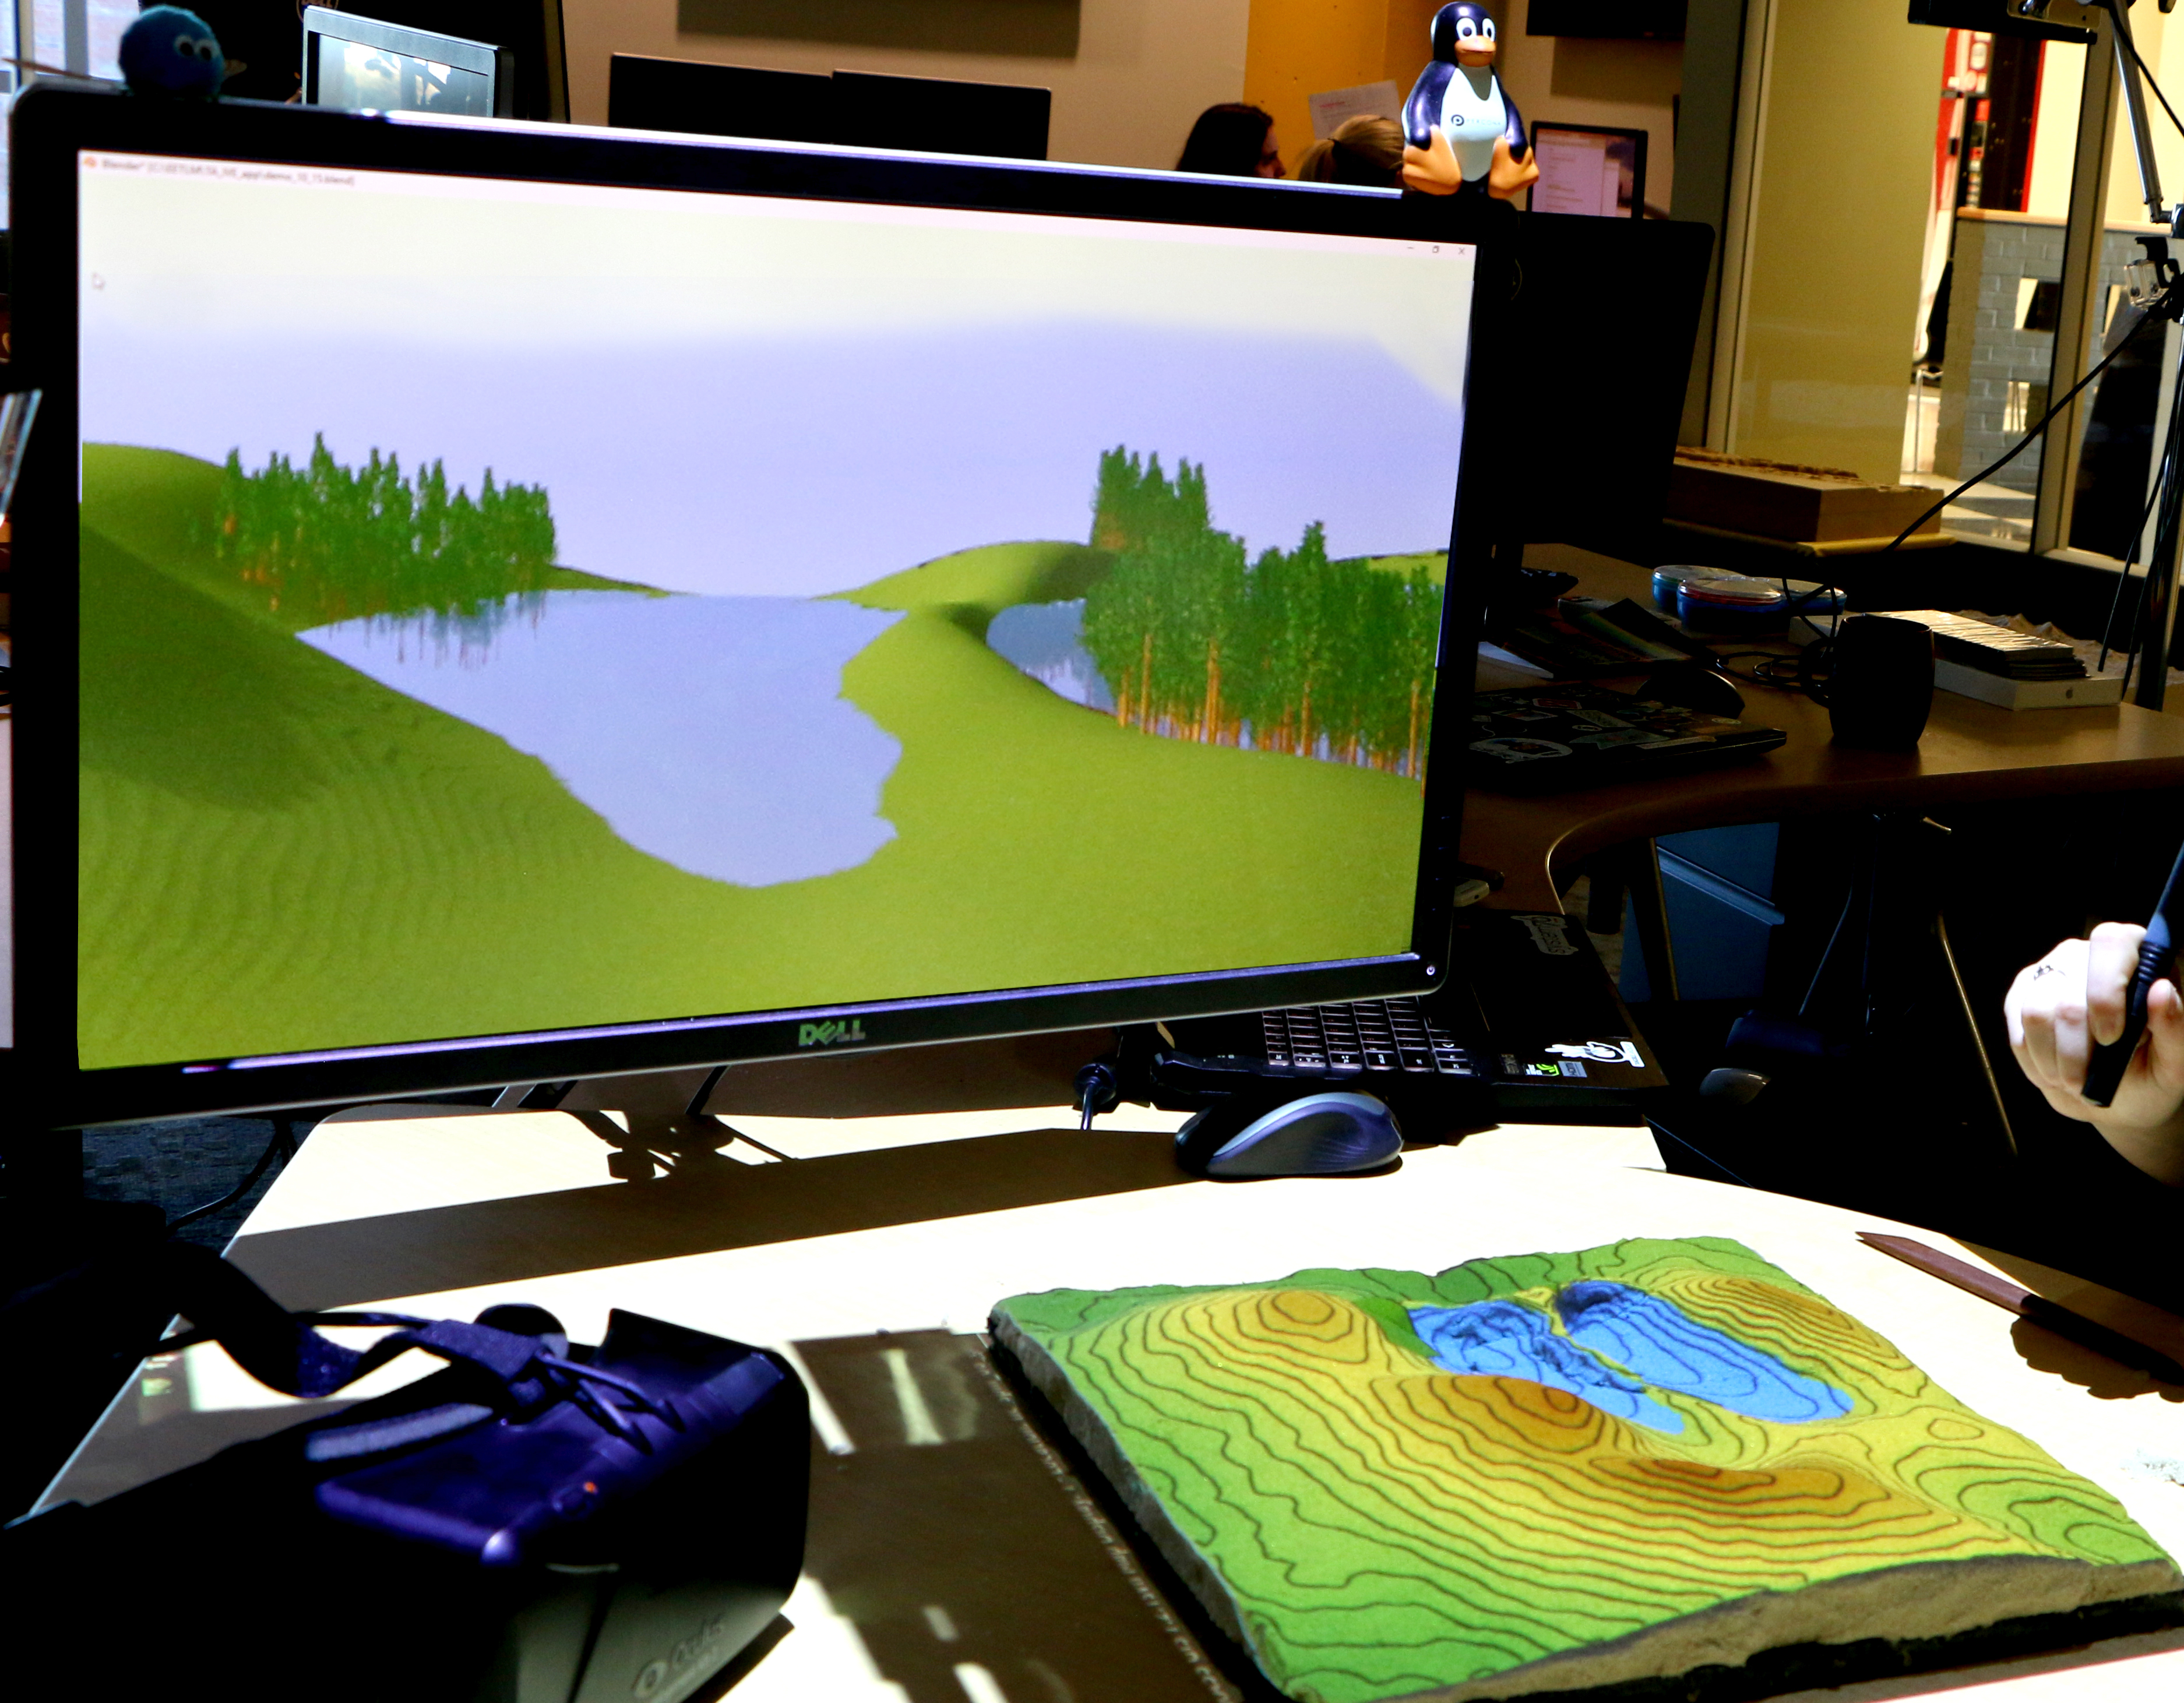
\includegraphics[width=0.49\textwidth]{images/immersive/tl_vr_demo_9.jpg}\\
%%
%\includegraphics[width=0.49\textwidth]{images/immersive/tl_vr_demo_5.jpg} &
%\includegraphics[width=0.49\textwidth]{images/immersive/tl_vr_demo_10.jpg}\\
%%
%\bottomrule
%\end{tabular}
%\label{table:tl_demo} 
%\end{table*}

% RESEARCH QUESTIONS
\subsection{Research objectives}
Many of the theoretical underpinnings of tangibles 
remain unproven and unexplored. 
Do current approaches to tangible, embodied interfaces
really work as theorized? 
Can designers really model more intuitively and 
design more effectively with tangibles?
And how do tangibles mediate the design process?
%
In order to assess the effectiveness 
of tangible modeling for landscape architects 
we conducted a series of user studies
assessing how well participants performed
basic landscape design tasks 
-- topographic modeling, cut-and-fill analysis, and water flow modeling --
using Tangible Landscape.\\

Our research objectives were to:
%
\begin{itemize}
% Performance
\item Assess how well landscape architects could perform basic design tasks using
a tangible interface for landscape modeling
% Process
\item Study how tangible interaction mediated
landscape architects' design process
\end{itemize}

\clearpage

% ---------------------------- TOPOGRAPHIC ---------------------------- 

\section{Topographic modeling}
%
One of the primary tasks of landscape architects is to design earthworks
\cite{Petschek2008,Strom2013}. 
% topographic data
Landscape architects work with topographic models 
derived from data collected by field surveys, airborne lidar, 
or photogrammetry with unmanned aerial systems.
% designing landforms
They design new landforms 
using analog methods -- such as 
drawing contours maps by hand and
hand sculpting physical topographic models in clay --
and digital methods -- such as 
drawing digital contour maps in CAD,
digitally sculpting surfaces in 3D modeling software. 
% analog
Analog methods for topographic modeling are typically used 
in the early, conceptual phases of the design process because 
they are considered more intuitive, but less precise than digital methods.
% digital
Digital methods for topographic modeling, on the other hand, 
can afford precise transformations and
dynamic modes of visualization such as 
3D orbiting, zooming, and ray traced shading.
% tangible
Theoretically tangible topographic modeling 
should combine affordances of both -- 
enabling natural sensing and manipulation
with enriched visualization.
% experiment
To assess the effectiveness tangibles
we conducted a topographic modeling experiment
comparing 
digital 3D modeling with Rhinoceros, 
analog modeling by hand, 
and tangible modeling with Tangible Landscape. 

\subsection{Methods}
% overview
In this experiment 
18 participants tried to accurately model a study landscape 
digitally, by hand, and with Tangible Landscape. 
% tasks
Participants were given three tasks -- 
to digitally sculpt a model of a landscape using the 3D modeling program Rhinoceros, 
to hand sculpt a model of a landscape in polymer-enriched sand,
and to sculpt a model of a landscape using Tangible Landscape.
% time limit 
They had 10 minutes to complete each task. 
The time limit was calibrated based on 
the time it took the research team 
to comfortably complete each task. 
% counterbalancing / order of tasks
The modeling tasks were reordered for each participant
to partially account for learning and fatigue
by counterbalancing the experiment using a Latin square design.
% assessment
Participants were asked to model the same landscape for each task 
so that their performance could be quantitatively assessed 
using spatial modeling, statistics, analysis, and simulation.
Their modeling processes were qualitatively assessed 
through direct observation
supported by photographic and video documentation. 
% interviews
After completing the tasks
the academics and professionals 
were interviewed. 
We intended to conduct semi-structured interviews 
with all of the participants, but
the students were too tired by the end of the experiment. 
% psychometric tests
Psychometric tests were not used
to assess spatial ability because
these do not address 
geographic scales,
spatial relations,
domain-specific knowledge and abilities 
\cite{Lee2009,Bednarz2011,Wakabayashi2011},
or embodied cognitive ability. 

% participants
\paragraph{Participants}
In order to compare the performance of novices and experts
we used graduate students, faculty, and professionals 
in architecture, landscape architecture, or geographic information science
for this study (see Table~\ref{table:participants}).
Of the 12 graduate students 6 were in the \nth{2} semester of the 
Master of Landscape Architecture program 
at North Carolina State University.
These students were just beginning to learn to read and manipulate contour lines 
in the class Landform, Site Grading, and Development Systems. 
%They had no experience with GIS, 3 credit hours of training in digital representation, 
%and no experience with Rhinoceros.
The other 6 graduate students were in the \nth{2} semester of the 
Master of Geospatial Information Science and Technology program 
at North Carolina State University.
%They had at least 9 credits hours of training in GIS, but 
%had no experience with contour maps, digital terrain modeling, or 3D modeling.
The other 6 participants were either landscape architecture faculty 
with professional experience or practicing professionals in landscape architecture 
from around the world. 
Of these 2 were experts in 3D modeling with over 10 years of experience 
using Rhinoceros and similar programs including Maya and 3ds Max. 
These experts felt comfortable and proficient modeling a wide variety of geometries 
and had developed unique, personalized, and highly adaptable workflows.

\begin{table}
\caption{Participants}
\ra{1.3}
\begin{tabular}{l <{\hspace{1em}} c <{\hspace{1em}} c}
\toprule
Group & No. & \mbox{3D expertise}\\
\midrule
Students & 12 & 0\\
Academics \& professionals & 6 & 2\\
\bottomrule
\end{tabular}
\label{table:participants} 
\end{table}

% digital modeling
\paragraph{Digital modeling}
Participants had 10 minutes 
to digitally model the study landscape in Rhinoceros 5, 
a non-uniform rational basis spline 
(NURBS) based 3D modeling program
designed for precise freeform curve and surface modeling \cite{Rhino}.
After 10 minutes of training 
participants modeled the study landscape as a NURBS surface 
by vertically translating control points (Fig.~\ref{fig:rhino}). 
They started with a flat NURBS surface that was 
divided into a 10 x 10 grid of control points.
As a reference their model space also included 
a locked representation of the study landscape as 3D contours. 
At any point participants could rebuild the surface 
with a higher density of control points for finer, more nuanced control. 
This method is relatively simple and 
analogous to basic actions in sculpture -- pushing and pulling. 
We developed and tested this method 
as a simple, straightforward technique for  
digital freeform surface modeling
that could be taught quickly, yet could produce an accurate model. 
Through testing we determined that 
novice users took approximately 10 minutes
to model the surface with a 10 x 10 grid of control points
before wanting to rebuild the surface with more control points.
% videos
See \url{https://youtu.be/dSyrHAuu698}
for a video demonstrating the training
and \url{https://youtu.be/vA1xwMSaGV4}
for a video demonstrating the digital 3D modeling task.

% choice of 3d modeling program
Different 3D modeling programs afford very different
interactions, modeling tools, data structures, and modes of representations. 
Developing a simple, intuitive modeling technique 
drove the choice of software in this study. 
After testing 3D modeling workflows in 
Rhinoceros, Vue, Maya, and SketchUp
we chose Rhinoceros 5 for this task because it 
is popular with designers such as architects, 
has a wide variety of modeling tools,
can precisely represent continuous surfaces, 
and has plugins for importing and exporting geographic data. 
To make a fair comparison 
between digital, analog, and tangible modeling,
the digital modeling technique 
needed to be relatively analogous to hand sculpting
-- i.e.~pushing and pulling rather than painting in 3D, 
drafting in 3D, or stacking voxels.

% analog modeling
\paragraph{Analog modeling}
After a brief explanation and demonstration
participants had 10 minutes to sculpt 
the study landscape in polymer-enriched sand 
by hand or with a wooden sculpting tool (Fig.~\ref{fig:analog}).  
They were given a CNC-routed model of the study landscape 
as a reference, a sculpting tool, and a 3D scale. 
Participants were shown how the 3D scale could be used to 
measure the height of the model. 
A lamp on the table cast shadows across the model for hillshading.
% videos
See \url{https://youtu.be/STYHUHNaWdY}
for a video demonstrating the analog 3D modeling task.

% tangible modeling
\paragraph{Tangible modeling}
After a minute long explanation and demonstration
participants had 10 minutes to sculpt
a projection-augmented, polymer-enriched sand model
of the study landscape 
either by hand or with a wooden sculpting tool 
(Fig.~\ref{fig:proj_aug}). 
Tangible Landscape was used to project 
an elevation map of the study landscape
with contours and a legend
onto participants' sand models as guide for sculpting. 
Participants were also given CNC routed reference model and 
a 3D scale ruled in map units. 
After an explanation of the contour map, elevation color table, and legend,
participants were shown how the 3D scale could be used to 
measure the elevation of their scale models.
% videos
See \url{https://youtu.be/1uEvzMJWh_E}
for a video demonstrating the tangible modeling task.

% data collection and analysis
\paragraph{Data collection and analysis}
We used Tangible Landscape to scan the finished models 
built using analog hand modeling and tangible modeling.
The scans were captured as point clouds, interpolated 
as digital elevation models 
using the regularized spline with tension method,
and stored as raster maps in a GRASS GIS database. 
The NURBS surfaces modeled in Rhinoceros 
were exported as raster elevation maps,
imported into GRASS GIS, randomly resampled, 
re-interpolated using the regularized spline with tension method, 
and stored as raster maps in a GRASS GIS database. 
The data from Rhinoceros 
was randomly resampled and re-interpolated to account for 
differences and irregularities in resolution, data density, and point spacing.
For each set of models -- digital, analog, and augmented --
we computed raster statistics (i.e.~per cell statistics), 
topographic and morphometric parameters, 
and simulated water flow.
%
% supplemental materials
Refer to the supplemental materials 
for more detailed description of the methodology
used in this study
\ref{appendix:methodology}.



% ---------------------------
\subsection{Results}

% overall results
Overall participants performed best with tangible modeling.
%
The 3D maps of raster statistics and geospatial analyses in
Table \ref{table:topography} 
show participants' performance with each technology.
%
When digitally modeling with Rhinoceros 
participants tended to 
create very approximate massings of the topography
with serious errors in the interior space and
with indistinct landforms
that only hinted at the morphology of the landscape.
%
When they sculpted by hand
their models tended to be descriptive -- 
differing substantially from the reference, but
accurately representing most of the landforms. 
%
Their performance improved 
with tangible modeling --
the resulting models
fit the reference better, 
had more defined topography, 
and accurately represented most of the landforms.

% group results
We used pairwise comparison to study 
how performance varied between 
novices and experts (Fig. \ref{fig:comparison}).
After analyzing all participants' performance
we compared students with academics and professionals. 
Then we compared landscape architecture students with GIS students.
Finally we compared academics and professionals 
with and without 3D modeling expertise.
%
When participants are analyzed as groups 
-- as GIS students, Landscape Architecture students, 
academics and professionals without 3D modeling expertise, 
and academics and professionals with 3D modeling expertise -- 
these trends generally still hold, 
albeit with some very important exceptions.
%
Unlike all other groups, 
the 3D modeling experts performed extremely well 
in the digital modeling task
with a very low standard deviation of difference, 
but still only hinted at the landforms. 
They, however, performed even better with tangible modeling,
accurately representing the landforms. 
%
See to the supplemental materials for more details
\ref{appendix:topographic_results}.
%
These results show 
tangible modeling should be 
should be a better, faster tool 
for quick modeling tasks such as rapid ideation. 
for both novices and experts.

\begin{figure*}[t]
%\begin{center}
\resizebox {\textwidth} {!} {\include*{comparison.tikz}}
\caption{Pairwise comparison of the mean digital elevation models by category of participants}
\label{fig:comparison}
%\end{center}
\end{figure*}

\include*{topographic}

% ---------------------------- CUT-FILL ---------------------------- 
\section{Cut-and-fill analysis}
% grading
When `grading' or earthmoving
landscape architects and civil engineers
seek to balance their sediment budget 
-- using as much cut (earth removed) 
as fill (earth deposited) --
to minimize the cost of transporting sediment to and from
the construction site.
% difference method
Because of the importance 
of balancing sediment budgets
we designed a real-time analytic 
for Tangible Landscape that 
maps the difference in elevation
before and after modification
to facilitate cut-and-fill analysis. 
% experiment
To test the effectiveness of this real-time analytic
we conducted a cut-and-fill experiment.

\subsection{Methods}
In the cut-and-fill experiment 
the same 18 participants were asked to use 
Tangible Landscape's difference analytic to model 
another study landscape
with a large central ridge 
flanked by valleys 
and a smaller, secondary ridge.
Participants had 10 minutes to model this region
in polymer-enriched sand using Tangible Landscape 
with the difference analytic (Table~\ref{fig:diff}). 
The difference between the reference elevation 
and the participant's modeled elevation
was computed in near real-time and projected onto the sand 
as an interactive guide.
The linear regression of the reference and scanned elevation maps 
was used to correct shifts in scanning and georeferencing. 
The difference showed where sand needs to added (blue) or removed (red) 
in order to match the reference landscape.
While this feedback should show users what to do next, 
it may provide too much data 
or be too challenging to rapidly parse and understand.
% video
See \url{https://youtu.be/Q3elMIRCYSk}
for a video demonstrating the 3D modeling task 
with the difference analytic.

\paragraph{Data collection and analysis}
The final scan of each model was stored in a 
GRASS GIS database for analysis. 
We used raster statistics, the difference in elevation, 
topographic parameters, and morphometric parameters
to compare the reference elevation 
and the set of modeled elevations. 
We computed 
the mean elevation,
the standard deviation of elevations, 
and the standard deviation of difference for the set.
To find the standard deviation of differences 
we first computed the difference 
between the reference elevation and each elevation 
and then used raster statistics 
to find the standard deviation of these differences.
We also computed the difference between the 
reference elevation and the mean elevation for the set. 
The reference elevation used in the difference calculation 
was rescaled and shifted based on the 
linear regression of the reference and mean elevation.
We computed the slope and landforms of the mean elevation. 
We also filmed each session, 
observed and took notes on participants' modeling processes, 
and interviewed participants.

\subsection{Results}
% table
The 3D maps of raster statistics and geospatial analyses in
Tables~\ref{table:difference_comparison}-\ref{table:difference_percent_cells} 
show participants' performance with the difference analytic.
% overview of results
Participants performed well with the difference analytic 
-- modeling simplified, 
but relatively accurate approximations of the landscape.
Participants with expertise in 3D modeling 
performed even better than other participants 
-- more accurately modeling the elevation and slopes,
but not the landforms. 
Since these models were sculpted in sand,
their edges tend to slump.
This caused systematic artifacts in the analysis like
low elevation values and steep slopes
along the borders. 
Based on interviews and observations
we found that the difference analytic enabled
a rapid, iterative process 
of modeling, learning from computational feedback, 
re-remodeling, etc.

%  mean
The mean elevation for this set of models
has the approximate shape of the reference elevation, 
but is much simpler, lacking many details. 
% stdev diff
The standard deviation of difference shows 
how consistently the models fit the reference. 
Overall participants performed well -- 
there was little deviation from the best fit. 
Participants tended to perform poorly 
near the edges of models, especially in the corners.
They also had trouble with the valleys 
and the low point by the secondary ridge.
% slope
The mean slope shows that participants tended to model 
overly steep slopes for the primary ridge -- exaggerating its form --
but tended not model steep enough slopes for the secondary ridge. 
% landforms
The mean landforms show that participants tended to 
clearly capture the central ridge and its spurs and
the secondary ridge and its valley, but missed the 
other valleys.
Hollows -- transitions between slopes, footslopes, and valleys -- 
on the mean landform map hint at these other 
valleys in the right locations.
% experts
The 3D modeling experts built more accurate models
with a lower standard deviation of differences 
and more accurate slopes. 
Since they did not, however, exaggerate the central ridge
and did not smooth its slopes, 
they did not cleanly represent this landform. 
The others built more exaggerated models 
that more clearly captured the main ridge.

% understanding volume
To successfully use the difference analytic 
participants had to think about topography as volume.
They had to either add or excavate sand to make the models match. 
One of the participants 
described modeling with the difference analytic
as a continual process of 'rebuilding to make it match.'
% iterative process
When interviewed
participants described an iterative process of 
continual refinement based on critical analysis 
-- similar to Sch{\"o}n's reflection-in-action \cite{Schon1983} --
but enhanced by computational feedback,
explaining that 
`because Tangible Landscape gives immediate results 
it encourages an iterative process.' 
See Table \ref{table:interviews} for select comments about this experiment.

% conclusions
The difference analytic is intuitive -- 
participants were able to learn how to use it effectively without training, 
producing good, albeit exaggerated approximations of the landscape. 
%
Their models tended to have key morphometric characteristics -- 
the primary ridge, its spurs, the low point, 
the secondary ridge, and one of the valleys -- 
but these characteristics tended to be 
either over- or under-exaggerated.

\include*{cut_fill}

%See to the supplemental materials for more details
%\ref{appendix:cut_fill_results}.


% ---------------------------- WATER FLOW ---------------------------- 
\section{Water flow modeling}

After a pilot study \cite{Harmon2016}
we conducted an experiment to study 
how water flow analytics 
mediate 3D spatial performance
when using a tangible interface for GIS.
%
This experiment was designed to study whether
participants could link form and process
using the water flow analytic -- to assess
how well they could understand the relationship 
between topographic form 
and the flow of water 
when using Tangible Landscape.

The same 18 participants were asked to model water flow 
across another region of Lake Raleigh Woods
using Tangible Landscape with the water flow analytic.
This region has a central ridge 
flanked by a large stream on one side 
and a small stream on the other.  
A third, smaller stream bisects the ridge.
Participants had 10 minutes to model water flow across this region
by sculpting polymer-enriched sand using Tangible Landscape 
with the water flow analytic. 
They sculpted sand models of the topography
to direct the simulated flow of water.  
Water flow was simulated in near real-time 
as a diffusive wave approximation of shallow water flow.
The module \textit{r.sim.water} \cite{r.sim.water}
uses a path sampling technique to solve the shallow water flow continuity equation \cite{Mitasova2004}.
Participants could switch between the precomputed reference water flow 
-- i.e.~their target -- 
and the water flow over their scanned model.
%
See \url{https://youtu.be/61hsXgb3MLY}
for a video demonstrating the 3D modeling task 
with the water flow analytic.




\subsection{Methods}



\subsection{Results}

\include*{water_flow}

\include*{interviews}




% ---------------------------- DISCUSSION ---------------------------- 
\section{Discussion}


% REFLECTIONS

% reflect on design implications
% performative design, parametric / generative design
% performance, process-based
% physical processes as design inspiration / media
% co-evolution
% cyborg ecologies vs cthuthonic

%With computational modeling, analysis and simulation designers can generate novel forms, explore parametric variations, and quantitatively test the performance of their designs. (ACADIA)

 %
%With this technology landscape architects and spatial scientists can collaboratively design through a seamless, rapid iterative process of intuitive ideation, geocomputational analysis, realistic rendering, and critical analysis. (ACADIA)



% ---------------------------- CONCLUSION ---------------------------- 

\section{Conclusion}


% EARTHWORKS, WATER, and EROSION
% Design implications, importance of topographic modeling in landscape architecture
% complex interaction of form and process

%%INTERACTION AND PERFORMANCE
%
%By naturally sketching in 3D, while learning from real-time analytical feedback 
%designers can work in a rapid, iterative design process 
%to quickly give their ideas form and test them.
%They can intuitively explore how form affects process. 
%With real-time geospatial simulations for example
%landscape architects can design high performance, process-based landscapes.
%With simulations seamlessly integrated into conceptual design
%physical processes like the flow of water 
%can play a generative role. 

%With computational modeling, analysis and simulation designers can generate novel forms, explore parametric variations, and quantitatively test the performance of their designs. (ACADIA)

 %
%With this technology landscape architects and spatial scientists can collaboratively design through a seamless, rapid iterative process of intuitive ideation, geocomputational analysis, realistic rendering, and critical analysis. (ACADIA)






\clearpage

\section{Conclusion}
This study proves that tangible landscape modeling
can be an effective landscape design tool
enabling a rapid, iterative design process and
enhancing spatial performance.

% role in design process
% design process

%% concept
%Tangible Landscape -- a tangible interface for GIS -- 
%enables natural 3D sketching. % 4D spatiotemporal sketching.

%% tangibles can enhance spatial performance
%Through a series of experiments
%we found that tangible interfaces for spatial modeling
%can enhance 3D spatial performance 
%in terms of speed, accuracy, and process. 
%% coupling
%By comparing digital, analog, and projection-augmented modeling 
%we found that coupling digital and physical models as a tangible interface 
%can combine the affordances of digital and analog tools
%-- enabling an embodied modeling process enriched with digital data --
%so that users can model intuitively, quickly, and precisely. 
%Even 3D modeling experts 
% performed better with the tangible interface 
%-- building more accurate models 
%that better represented the morphology of the landscape --
% because they could work faster
% creating and refining details sooner.
%% transfer
%They were able to transfer and effectively use the
%spatial skills and abilities they had developed through digital modeling
%with the tangible interface.
%% analytics
%We also found that tangible interaction with real-time geospatial analytics
%can encourage iterative modeling processes.
%With the real-time difference analytic and water flow simulation  
%users worked in rapid cycles of 
%sculpting and digitally informed critical analysis
%to build accurate models that
%correctly represented the topographic and hydrologic morphology.
%% process
%Through this embodied process of reflection-in-action 
%users were able to
%observe spatial patterns, forms, and processes, 
%generate and test hypotheses, 
%and draw inferences. 
%% cog offloading
%The experiments showed that users 
%were able to offload enough of the cognitive work 
%of sensing and manipulating space
%onto their bodies
%that they could understand the
%computational analytics
%and adaptively re-strategize.
%% future research
%Further experiments are needed
%to explore the role of 
%spatial cognition, affect, motivation, and metacognition 
%in tangible modeling.
%
%% summary
%The experiments show that Tangible Landscape,
%a tangible interface for GIS, 
%works as theorized and designed -- 
%coupling a physical and digital model of a landscape
%enables users to 
%cognitively grasp topography,
%intuitively shape and interact with multidimensional space, 
%and offload enough cognitive work to understand 
%real-time geospatial analytics. 
%% process 
%With Tangible Landscape users can intuitively interact with 
%spatial data and scientific models using their bodies. 
%% users
%While novices should be able to effectively learn about 
%multidimensional space and
%rapidly improve their spatial abilities 
%with Tangible Landscape, 
%experts can effectively use it to 
%rapidly develop, prototype, and test 
%hypotheses about space and spatiotemporal processes.


% QUOTE
%'bridge the division between physical and digital forms and potentially to revolutionize the current design process' \cite{Ishii2004}.


% ---------------------------- SUPPLEMENTAL MATERIAL ---------------------------- 

%https://us.sagepub.com/en-us/nam/supplementary-files-on-sage-journals-sj-guidelines-for-authors

\begin{sm}
%\noindent
Python scripts for data processing and analysis: \\
\noindent
\url{https://github.com/baharmon/tangible_topography}

\noindent
Data, results, and methods: \url{https://osf.io/82gst/}

\noindent
Website: \url{http://tangible-landscape.github.io/}

\noindent
GitHub: \url{https://github.com/tangible-landscape}

\noindent
Wiki: \url{https://github.com/tangible-landscape/grass-tangible-landscape/wiki}

\noindent
Videos: \url{youtube.com/c/NCSUGeoForAllLab} 








\end{sm}


% ------------------- GUIDELINES ----------------------- 

%https://us.sagepub.com/en-us/nam/international-journal-of-architectural-computing/journal202464#submission-guidelines

















% ---------------------------- TEMPLATE ---------------------------- 

%\section{Template}
%\begin{enumerate}
%\item[(i)] ...
%\item[(ii)] ...
%\item[(iii)] ...
%\end{enumerate}
%
%\begin{figure*}
%%\setlength{\fboxsep}{0pt}%
%%\setlength{\fboxrule}{0pt}%
%\begin{center}
%\end{center}
%\caption{...}
%\label{F1}
%\end{figure*}
%
%Figure~\ref{F1}. You must select options for the trim/text area and
%the reference style of the journal you are submitting to.
%The choice of \verb+options+ are listed in Table~\ref{T1}.
%
%\begin{table}[h]
%\small\sf\centering
%\caption{Table.\label{T1}}
%\begin{tabular}{lll}
%\toprule
%Header 1 & Header 2 & Header 3\\
%\midrule
%\texttt{...}& ... & ....\\
%\bottomrule
%\end{tabular}\\ %[15pt] % for vspace between tabulars
%\end{table}




% ---------------------------- ENDNOTES ---------------------------- 

%\subsection{Endnotes}
%Most \textit{SAGE} journals use endnotes rather than footnotes, so any notes should be coded as \verb+\endnote{<Text>}+.
%Place the command \verb+\theendnotes+ just above the Reference section to typeset the endnotes.
%To avoid any confusion for papers that use Vancouver style references,  footnotes/endnotes should be edited into the text.


% ---------------------------- SUPPLEMENTAL MATERIAL ---------------------------- 

%\begin{verbatim}
%\begin{sm}
%To typeset a
%  "Supplemental material" section.
%\end{sm}
%\end{verbatim}

% ---------------------------- ACKNOWLEDGEMENTS---------------------------- 

% Gene Bressler

% Art Rice

% GRASS GIS Dev Community

% Blender Dev Community

%\begin{acks}
%This class file was developed by Sunrise Setting Ltd,
%Brixham, Devon, UK.\\
%Website: \url{http://www.sunrise-setting.co.uk}
%\end{acks}

% ---------------------------- BIBLIOGRAPHY ---------------------------- 

%\bibliographystyle{SageH}
\bibliographystyle{SageV}
\bibliography{tangible_topography.bib} 

\end{document}
